
%% L3-project-paper-template.tex
%% v1.1
%% Dec, 2022
%% Craig Stewart
%% for Durham University, Computer Science Project paper templates
%% contact craig.d.stewart at durham.ac.uk for support
%%
%% Based on IEEE Template: bare_jrnl_compsoc.tex, V1.4b, by Michael Shell
%%
%% Notice from original IEEE Template:
%%*************************************************************************
%% Legal Notice:
%% This code is offered as-is without any warranty either expressed or
%% implied; without even the implied warranty of MERCHANTABILITY or
%% FITNESS FOR A PARTICULAR PURPOSE! 
%% User assumes all risk.
%% In no event shall the IEEE or any contributor to this code be liable for
%% any damages or losses, including, but not limited to, incidental,
%% consequential, or any other damages, resulting from the use or misuse
%% of any information contained here.
%%
%% All comments are the opinions of their respective authors and are not
%% necessarily endorsed by the IEEE.
%%
%% This work is distributed under the LaTeX Project Public License (LPPL)
%% ( http://www.latex-project.org/ ) version 1.3, and may be freely used,
%% distributed and modified. A copy of the LPPL, version 1.3, is included
%% in the base LaTeX documentation of all distributions of LaTeX released
%% 2003/12/01 or later.
%% Retain all contribution notices and credits.
%% ** Modified files should be clearly indicated as such, including  **
%% ** renaming them and changing author support contact information. **
%%*************************************************************************


\documentclass[10pt,journal,compsoc]{IEEEtran}

% Some very useful LaTeX packages include:
% (uncomment the ones you want to load)
\usepackage{appendix}
\usepackage{float}

%% ---------------------------------------------- START OF USEFUL PACKAGES ----------------------------------------------

%\usepackage{ifpdf}
% Heiko Oberdiek's ifpdf.sty is very useful if you need conditional
% compilation based on whether the output is pdf or dvi.
% usage:
% \ifpdf
%   % pdf code
% \else
%   % dvi code
% \fi
% The latest version of ifpdf.sty can be obtained from:
% http://www.ctan.org/pkg/ifpdf
% Also, note that IEEEtran.cls V1.7 and later provides a builtin
% \ifCLASSINFOpdf conditional that works the same way.
% When switching from latex to pdflatex and vice-versa, the compiler may
% have to be run twice to clear warning/error messages.


% *** CITATION PACKAGES ***
%
\ifCLASSOPTIONcompsoc
  % IEEE Computer Society needs nocompress option
  % requires cite.sty v4.0 or later (November 2003)
  \usepackage[nocompress]{cite}
\else
  % normal IEEE
  \usepackage{cite}
\fi
% cite.sty was written by Donald Arseneau
% V1.6 and later of IEEEtran pre-defines the format of the cite.sty package
% \cite{} output to follow that of the IEEE. Loading the cite package will
% result in citation numbers being automatically sorted and properly
% "compressed/ranged". e.g., [1], [9], [2], [7], [5], [6] without using
% cite.sty will become [1], [2], [5]--[7], [9] using cite.sty. cite.sty's
% \cite will automatically add leading space, if needed. Use cite.sty's
% noadjust option (cite.sty V3.8 and later) if you want to turn this off
% such as if a citation ever needs to be enclosed in parenthesis.
% cite.sty is already installed on most LaTeX systems. Be sure and use
% version 5.0 (2009-03-20) and later if using hyperref.sty.
% The latest version can be obtained at:
% http://www.ctan.org/pkg/cite
% The documentation is contained in the cite.sty file itself.
%
% Note that some packages require special options to format as the Computer
% Society requires. In particular, Computer Society  papers do not use
% compressed citation ranges as is done in typical IEEE papers
% (e.g., [1]-[4]). Instead, they list every citation separately in order
% (e.g., [1], [2], [3], [4]). To get the latter we need to load the cite
% package with the nocompress option which is supported by cite.sty v4.0
% and later. Note also the use of a CLASSOPTION conditional provided by
% IEEEtran.cls V1.7 and later.


% *** GRAPHICS RELATED PACKAGES ***
%
\ifCLASSINFOpdf
  \usepackage[pdftex]{graphicx}
  % declare the path(s) where your graphic files are
  % \graphicspath{{../pdf/}{../jpeg/}}
  % and their extensions so you won't have to specify these with
  % every instance of \includegraphics
  % \DeclareGraphicsExtensions{.pdf,.jpeg,.png}
\else
  % or other class option (dvipsone, dvipdf, if not using dvips). graphicx
  % will default to the driver specified in the system graphics.cfg if no
  % driver is specified.
  % \usepackage[dvips]{graphicx}
  % declare the path(s) where your graphic files are
  % \graphicspath{{../eps/}}
  % and their extensions so you won't have to specify these with
  % every instance of \includegraphics
  % \DeclareGraphicsExtensions{.eps}
\fi
% graphicx was written by David Carlisle and Sebastian Rahtz. It is
% required if you want graphics, photos, etc. graphicx.sty is already
% installed on most LaTeX systems. The latest version and documentation
% can be obtained at: 
% http://www.ctan.org/pkg/graphicx
% Another good source of documentation is "Using Imported Graphics in
% LaTeX2e" by Keith Reckdahl which can be found at:
% http://www.ctan.org/pkg/epslatex
%
% latex, and pdflatex in dvi mode, support graphics in encapsulated
% postscript (.eps) format. pdflatex in pdf mode supports graphics
% in .pdf, .jpeg, .png and .mps (metapost) formats. Users should ensure
% that all non-photo figures use a vector format (.eps, .pdf, .mps) and
% not a bitmapped formats (.jpeg, .png). The IEEE frowns on bitmapped formats
% which can result in "jaggedy"/blurry rendering of lines and letters as
% well as large increases in file sizes.
%
% You can find documentation about the pdfTeX application at:
% http://www.tug.org/applications/pdftex


% *** MATH PACKAGES ***
%
%\usepackage{amsmath}
% A popular package from the American Mathematical Society that provides
% many useful and powerful commands for dealing with mathematics.
%
% Note that the amsmath package sets \interdisplaylinepenalty to 10000
% thus preventing page breaks from occurring within multiline equations. Use:
%\interdisplaylinepenalty=2500
% after loading amsmath to restore such page breaks as IEEEtran.cls normally
% does. amsmath.sty is already installed on most LaTeX systems. The latest
% version and documentation can be obtained at:
% http://www.ctan.org/pkg/amsmath


% *** SPECIALIZED LIST PACKAGES ***
%
%\usepackage{algorithmic}
% algorithmic.sty was written by Peter Williams and Rogerio Brito.
% This package provides an algorithmic environment fo describing algorithms.
% You can use the algorithmic environment in-text or within a figure
% environment to provide for a floating algorithm. Do NOT use the algorithm
% floating environment provided by algorithm.sty (by the same authors) or
% algorithm2e.sty (by Christophe Fiorio) as the IEEE does not use dedicated
% algorithm float types and packages that provide these will not provide
% correct IEEE style captions. The latest version and documentation of
% algorithmic.sty can be obtained at:
% http://www.ctan.org/pkg/algorithms
% Also of interest may be the (relatively newer and more customizable)
% algorithmicx.sty package by Szasz Janos:
% http://www.ctan.org/pkg/algorithmicx


% *** ALIGNMENT PACKAGES ***
%
%\usepackage{array}
% Frank Mittelbach's and David Carlisle's array.sty patches and improves
% the standard LaTeX2e array and tabular environments to provide better
% appearance and additional user controls. As the default LaTeX2e table
% generation code is lacking to the point of almost being broken with
% respect to the quality of the end results, all users are strongly
% advised to use an enhanced (at the very least that provided by array.sty)
% set of table tools. array.sty is already installed on most systems. The
% latest version and documentation can be obtained at:
% http://www.ctan.org/pkg/array


% IEEEtran contains the IEEEeqnarray family of commands that can be used to
% generate multiline equations as well as matrices, tables, etc., of high
% quality.


% *** SUBFIGURE PACKAGES ***
%\ifCLASSOPTIONcompsoc
%  \usepackage[caption=false,font=footnotesize,labelfont=sf,textfont=sf]{subfig}
%\else
%  \usepackage[caption=false,font=footnotesize]{subfig}
%\fi
% subfig.sty, written by Steven Douglas Cochran, is the modern replacement
% for subfigure.sty, the latter of which is no longer maintained and is
% incompatible with some LaTeX packages including fixltx2e. However,
% subfig.sty requires and automatically loads Axel Sommerfeldt's caption.sty
% which will override IEEEtran.cls' handling of captions and this will result
% in non-IEEE style figure/table captions. To prevent this problem, be sure
% and invoke subfig.sty's "caption=false" package option (available since
% subfig.sty version 1.3, 2005/06/28) as this is will preserve IEEEtran.cls
% handling of captions.
% Note that the Computer Society format requires a sans serif font rather
% than the serif font used in traditional IEEE formatting and thus the need
% to invoke different subfig.sty package options depending on whether
% compsoc mode has been enabled.
%
% The latest version and documentation of subfig.sty can be obtained at:
% http://www.ctan.org/pkg/subfig


% *** FLOAT PACKAGES ***
%
%\usepackage{fixltx2e}
% fixltx2e, the successor to the earlier fix2col.sty, was written by
% Frank Mittelbach and David Carlisle. This package corrects a few problems
% in the LaTeX2e kernel, the most notable of which is that in current
% LaTeX2e releases, the ordering of single and double column floats is not
% guaranteed to be preserved. Thus, an unpatched LaTeX2e can allow a
% single column figure to be placed prior to an earlier double column
% figure.
% Be aware that LaTeX2e kernels dated 2015 and later have fixltx2e.sty's
% corrections already built into the system in which case a warning will
% be issued if an attempt is made to load fixltx2e.sty as it is no longer
% needed.
% The latest version and documentation can be found at:
% http://www.ctan.org/pkg/fixltx2e

%\usepackage{stfloats}
% stfloats.sty was written by Sigitas Tolusis. This package gives LaTeX2e
% the ability to do double column floats at the bottom of the page as well
% as the top. (e.g., "\begin{figure*}[!b]" is not normally possible in
% LaTeX2e). It also provides a command:
%\fnbelowfloat
% to enable the placement of footnotes below bottom floats (the standard
% LaTeX2e kernel puts them above bottom floats). This is an invasive package
% which rewrites many portions of the LaTeX2e float routines. It may not work
% with other packages that modify the LaTeX2e float routines. The latest
% version and documentation can be obtained at:
% http://www.ctan.org/pkg/stfloats
% Do not use the stfloats baselinefloat ability as the IEEE does not allow
% \baselineskip to stretch. Authors submitting work to the IEEE should note
% that the IEEE rarely uses double column equations and that authors should try
% to avoid such use. Do not be tempted to use the cuted.sty or midfloat.sty
% packages (also by Sigitas Tolusis) as the IEEE does not format its papers in
% such ways.
% Do not attempt to use stfloats with fixltx2e as they are incompatible.
% Instead, use Morten Hogholm'a dblfloatfix which combines the features
% of both fixltx2e and stfloats:
%
% \usepackage{dblfloatfix}
% The latest version can be found at:
% http://www.ctan.org/pkg/dblfloatfix


%\ifCLASSOPTIONcaptionsoff
%  \usepackage[nomarkers]{endfloat}
% \let\MYoriglatexcaption\caption
% \renewcommand{\caption}[2][\relax]{\MYoriglatexcaption[#2]{#2}}
%\fi
% endfloat.sty was written by James Darrell McCauley, Jeff Goldberg and 
% Axel Sommerfeldt. This package may be useful when used in conjunction with 
% IEEEtran.cls'  captionsoff option. Some IEEE journals/societies require that
% submissions have lists of figures/tables at the end of the paper and that
% figures/tables without any captions are placed on a page by themselves at
% the end of the document. If needed, the draftcls IEEEtran class option or
% \CLASSINPUTbaselinestretch interface can be used to increase the line
% spacing as well. Be sure and use the nomarkers option of endfloat to
% prevent endfloat from "marking" where the figures would have been placed
% in the text. The two hack lines of code above are a slight modification of
% that suggested by in the endfloat docs (section 8.4.1) to ensure that
% the full captions always appear in the list of figures/tables - even if
% the user used the short optional argument of \caption[]{}.
% IEEE papers do not typically make use of \caption[]'s optional argument,
% so this should not be an issue. A similar trick can be used to disable
% captions of packages such as subfig.sty that lack options to turn off
% the subcaptions:
% For subfig.sty:
% \let\MYorigsubfloat\subfloat
% \renewcommand{\subfloat}[2][\relax]{\MYorigsubfloat[]{#2}}
% However, the above trick will not work if both optional arguments of
% the \subfloat command are used. Furthermore, there needs to be a
% description of each subfigure *somewhere* and endfloat does not add
% subfigure captions to its list of figures. Thus, the best approach is to
% avoid the use of subfigure captions (many IEEE journals avoid them anyway)
% and instead reference/explain all the subfigures within the main caption.
% The latest version of endfloat.sty and its documentation can obtained at:
% http://www.ctan.org/pkg/endfloat
%
% The IEEEtran \ifCLASSOPTIONcaptionsoff conditional can also be used
% later in the document, say, to conditionally put the References on a 
% page by themselves.


% *** PDF, URL AND HYPERLINK PACKAGES ***
%
%\usepackage{url}
% url.sty was written by Donald Arseneau. It provides better support for
% handling and breaking URLs. url.sty is already installed on most LaTeX
% systems. The latest version and documentation can be obtained at:
% http://www.ctan.org/pkg/url
% Basically, \url{my_url_here}.

%% ---------------------------------------------- END OF USEFUL PACKAGES ----------------------------------------------



% *** Do not adjust lengths that control margins, column widths, etc. ***
% *** Do not use packages that alter fonts (such as pslatex).         ***

% correct bad hyphenation here
\hyphenation{op-tical net-works semi-conduc-tor}


\begin{document}
%
% paper title
% Titles are generally capitalized except for words such as a, an, and, as,
% at, but, by, for, in, nor, of, on, or, the, to and up, which are usually
% not capitalized unless they are the first or last word of the title.
% Linebreaks \\ can be used within to get better formatting as desired.
% Do not put math or special symbols in the title.
\title{A Cryptanalysis of Retro Block Ciphers}
%
%
% author  

\author{Student Name: A.I. Johnstone\\Supervisor Name: K. Southern\\
Submitted as part of the degree of BSc Computer Science to the\\
Board of Examiners in the Department of Computer Sciences, Durham University
}


% The paper headers
\markboth{DURHAM UNIVERSITY, DEPARTMENT OF COMPUTER SCIENCE}%
{Shell \MakeLowercase{\textit{et al.}}}

\IEEEtitleabstractindextext{%
\begin{abstract}
Testing the limits of past and present encryption methods is a key area within cryptography that ensures the security of the working world. New ways of attacking ciphers are constantly being developed; however, this paper will discuss a potentially powerful yet overlooked boomerang-based method known as a sandwich attack, which was created in 2010 and has barely been used since. Although originally designed to break the KASUMI block cipher the sandwich attack has not been utilised on more robust block ciphers and so the aim of this paper is to discuss the research question: is a sandwich attack a feasible method for breaking the GOST block cipher. In order to establish whether a sandwich attack is an efficient method to use against GOST, a ground-up style approach is taken in this paper, starting from a replication of a sandwich attack on KASUMI and a boomerang attack on GOST, which are both then used as a platform to build a sandwich attack on GOST. Although the attack on KASUMI could be successfully replicated, the results for the boomerang attack on GOST could not be, however, with a slight adjustment to the differentials comparable results could be achieved. Utilising both of these implementations, it was established that a sandwich attack on GOST would in fact be a feasibly efficient method through the use of truncated differentials, as this allowed the sandwich distinguisher to be created without adding extra complexity. Although this has not been tested experimentally, the results acquired from theory testing show good promise and suggest that a sandwich attack on GOST would be no more complex than the standard boomerang attack.
\end{abstract}

\begin{IEEEkeywords}

\end{IEEEkeywords}}

%% --------------------------------------------- DO NOT CHANGE ---------------------------------------------

% make the title area
\maketitle


% To allow for easy dual compilation without having to reenter the
% abstract/keywords data, the \IEEEtitleabstractindextext text will
% not be used in maketitle, but will appear (i.e., to be "transported")
% here as \IEEEdisplaynontitleabstractindextext when the compsoc 
% or transmag modes are not selected <OR> if conference mode is selected 
% - because all conference papers position the abstract like regular
% papers do.
\IEEEdisplaynontitleabstractindextext
% \IEEEdisplaynontitleabstractindextext has no effect when using
% compsoc or transmag under a non-conference mode.
% For peer review papers, you can put extra information on the cover
% page as needed:
% \ifCLASSOPTIONpeerreview
% \begin{center} \bfseries EDICS Category: 3-BBND \end{center}
% \fi
%
% For peerreview papers, this IEEEtran command inserts a page break and
% creates the second title. It will be ignored for other modes.
\IEEEpeerreviewmaketitle

\IEEEraisesectionheading{\section{Introduction}\label{sec:introduction}}
% Computer Society journal (but not conference!) papers do something unusual
% with the very first section heading (almost always called "Introduction").
% They place it ABOVE the main text! IEEEtran.cls does not automatically do
% this for you, but you can achieve this effect with the provided
% \IEEEraisesectionheading{} command. Note the need to keep any \label that
% is to refer to the section immediately after \section in the above as
% \IEEEraisesectionheading puts \section within a raised box.

%% --------------------------------------------- DO NOT CHANGE ---------------------------------------------




% The very first letter is a 2 line initial drop letter followed
% by the rest of the first word in caps (small caps for compsoc).
% 
% form to use if the first word consists of a single letter:
% \IEEEPARstart{A}{demo} file is ....
% 
% Here we have the typical use of a "T" for an initial drop letter
% and "HIS" in caps to complete the first word.
\IEEEPARstart{A}{dvances} in modern technology have meant that there is a constant need for encryption within our everyday lives. Subsequently these encryption methods have also needed to become more and more secure as attacks from hostile users have become increasingly advanced. As such the field of cryptography is always trying to find new ways to ensure security or conversely find new ways to breach this security so that they can stay ahead of malicious adversaries.

This work hopes to extend the studies surrounding the generation of best known attacks specifically looking at block cipher encryption. We achieve this by utilising a number of existing techniques and ciphers to create a platform from which we create a new attack on a retro block cipher. We then attempt to show that this new method is at least as good as existing methods with the potential to be a new best known attack. In addition to this we also explore a combination of methods which, although have appeared in previous research (\cite{Sun_Gerault_Wang_Wang_2020}, \cite{fse-2007-3268}, \cite{fse-2004-3110}), have not been applied in the same context as in this project. 

\subsection{Deliverables}
The research question asked in this paper is: 'Is a sandwich attack a feasible method for breaking the GOST block cipher?'

To try and answer this question a number of project deliverables were established and categorised into basic, intermediate and advanced deliverables. 

The basic deliverables were to replicate results from existing work notably, to replicate the results of a sandwich attack on KASUMI from \cite{jofc-2014-25962} and to replicate a related-key boomerang attack on GOST from \cite{cryptoeprint:2010/111}. The purpose of replicating the results from \cite{jofc-2014-25962} was to establish that the sandwich attack was in fact a correct method and could produce repeatable results. We were able to reproduce the results from \cite{jofc-2014-25962} by utilising the basic pseudocode provided \cite{jofc-2014-25962} which was then translated into Python alongside using a modified version of the KASUMI implementation from \cite{asecuritysite_82320}. The purpose of replicating the results from \cite{cryptoeprint:2010/111} was to gain a better understanding of the GOST block cipher and also to look at how the boomerang attack worked so as to better understand how to implement a sandwich attack. We were unable to directly achieve the same results as in \cite{cryptoeprint:2010/111} as we experienced some issues regarding the provided differentials, despite the provided differentials being the same as those used in other papers (e.g. \cite{inproceedings}) we were unable to get them to work. However, we did manage to get comparable results after adjusting the differentials, translating the pseudocode from \cite{cryptoeprint:2010/111} to Python and utilising an adapted version of GOST from \cite{githubGitHubBozhuGOSTPython}. The reason for replicating the results from two papers was to allow for us to gain a deeper understanding of how all of the key components needed to answer the research question worked and how they could later be combined.

The intermediate deliverable was to establish whether a sandwich attack on GOST would be feasible in theory based on its computational complexity. After establishing where to put the 'sandwich layer' we were able to work out that if a truncated differential was used then there was no additional work required to create the sandwich distinguisher compared to the boomerang distinguisher meaning that in theory the sandwich attack on GOST should be no more computationally complex than a related-key boomerang attack. This lead us to conclude that the sandwich attack could be a feasible method for breaking the GOST block cipher and subsequently answering the research question.

In the initial plan for this project two advanced deliverables were presented however they were dependent on the whether the intermediate deliverable was successful. The first advanced deliverable was for if we were able to show that in theory the sandwich attack was somewhat feasible meaning we would then go on to implement the attack to see if we could prove our results experimentally. The second advanced deliverable was for the scenario where a sandwich attack on GOST proved to be infeasible and so rather than attempting to implement the attack (as this would be pointless given that it is more complex than the existing related-key boomerang attack) we would instead add to the existing documentation of the sandwich attack providing more detailed descriptions and pseudocode for it. However, due to issues in the project regarding incomplete and outdated resources as well as implementation issues, the project fell behind schedule and subsequently we were unable to attempt any of the advanced deliverables.

\section{Related Work}
In this section a commentary of existing papers surrounding the subject area of this project will be presented, initially discussing and defining some baseline terms that are then expanded upon and developed into techniques that have been used in this project.
\subsection{Term definition}
To be able to gain an understanding of some of the more complex techniques used in this project a selection of useful terms have been provided below.
\subsubsection{Feistel Cipher}
When constructing a block cipher, it is common for the ‘main’ encryption part of the machine to be created using a Feistel cipher \cite{nachef2017feistel}. Named and designed by Horst Feistel, who did pioneering research whilst working for IBM, a Feistel cipher (also called a Feistel network) is a symmetric key algorithm that splits one of its inputs in half and then performs multiple ‘rounds’ on it and its second input, known as the key, to encrypt the original input. Within each round half of the split input is passed through a pseudorandom function, called the round function, alongside the key to ‘scramble’ the bits of the input half. The other half is then XOR’ed with the output from the round function and finally, the halves are swapped (left becomes right and right becomes left). Figure \ref{fig:fn} showcases the process of performing the round function on a Feistel network.

\begin{figure}[hbt!]
    \centering
    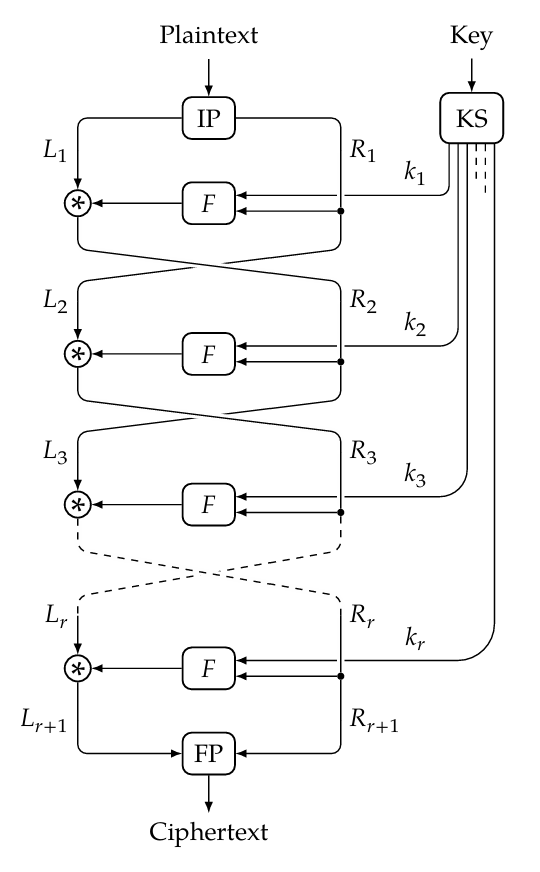
\includegraphics[width=0.5\linewidth]{Figures/fn.png}
    \caption{A diagram showing the schema of a Feistel cipher \cite{cryptoeprint:2016/1171-141-29}}
    \label{fig:fn}
\end{figure}
 

\subsubsection{S-Boxes}
Used in block ciphers to help obey Shannon’s property of confusion \cite{Anderson2008}, substitution boxes (S-boxes) are mathematically non-linear vectorial Boolean functions \cite{Carlet_2010}. However, in general, an S-box takes some number of input bits, m, and transforms them into some number of output bits, n. In this instance m doesn’t have to be equal to n for example DES takes a 6-bit input and produces a 4-bit output \cite{5389567}. S-boxes are used to help obscure the relationship between the plaintext and the ciphertext and to provide nonlinearity so that a block cipher cannot be trivially decrypted.

\subsection{Block Ciphers}
A key part of this project involves analysing block ciphers which are a type of private key cryptosystem that operate on fixed-length groups of bits, known as blocks \cite{cryptoeprint:2016/1171}. These block ciphers take a binary input string and then use an operation, for example, a Feistel cipher, to encrypt this input using a chosen second input called a key. In cryptography, these inputs are known as plaintexts and the outputs are called ciphertexts. Within this paper there are two primary block ciphers that are looked at however for ease of understanding this section mentions three.
\subsubsection{DES}
The Data Encryption Standard (DES) (First released in FIPS-46) is a block cipher developed in the early 1970s by IBM that utilises a balanced Feistel network of 16 rounds to encrypt 64-bit data blocks using a 56-bit key \cite{pub1999data}. Although originally being derived from the block cipher Lucifer, developed by Horst Feistel, DES was modified by the NSA (National Security Agency) to be more resistant to differential attacks before it was accepted as a national encryption standard in 1976  \cite{5389567}. Despite being more resistant to differential cryptanalysis, DES was also made to be weaker against brute force attacks by the NSA as they wanted to be able to break DES if it ever became necessary. Although upon release DES was known to not be completely secure it has since been proven that it is no longer a viable method of encryption. Notably in 1998 the EFF DES cracker (aka Deep Crack) \cite{10.5555/551916} could brute force a DES key in a matter of days. Hence in 2005 it was withdrawn from the encryption standard and replaced with a new block cipher called AES (Advanced Encryption Standard) \cite{daemen1999aes}. Despite this, some alternate versions of DES exist that are still considered secure such as TripleDES \cite{233626}. Although not used as an encryption standard any more DES is still an area of interest for researchers as it can give them a reliable benchmark for new attacks or potentially provide them with information about how AES will react to an attack. Although this project does not directly use DES, it can still be useful to use as a comparative benchmark for the proposed attacks as significantly more research has been done on DES compared to KASUMI or GOST.
\subsubsection{GOST}
GOST is a Soviet and Russian government standard symmetric key block cipher developed in 1989 (originally called Magma) \cite{rfc5830} but that has since had revisions and is still used today (now called Kuznyechik) \cite{rfc7801}. GOST (an acronym derived from gosudarstvennyy standard which translates to government standard) is similar to DES in that it is a 64-bit block size and utilises a Feistel network however some of the main differences between the two ciphers are listed below:
\begin{itemize}
    \item GOST uses a key size of 256-bits
    \item GOST uses 32 rounds of the Feistel function
    \item The S-boxes of GOST take a 4-bit input and produce a 4-bit output
    \item The S-boxes of GOST can be changed
\end{itemize}

Despite these differing factors appearing to make GOST a more secure cipher compared to DES, it was found in 2011 that GOST could be broken quite easily and was even called a ‘deeply flawed cipher’ by Nicolas Courtois \cite{cryptoeprint:2011/211}. 
Although GOST has been considered broken, the attack that would perform this is infeasible. This is why GOST has been chosen for this project as we would like to see if a sandwich attack can either further break GOST or provide a more feasible attack on it. Alongside choosing GOST we are also going to choose the S-boxes defined in the original publication of GOST \cite{rfc8891} as this should provide the best comparison to the first ‘retro’ version of GOST (aka Magma). Although this will later prove unnecessary as the related-key boomerang attack from which we build a sandwich attack on is s-box agnostic.
\subsubsection{KASUMI}
KASUMI is a Feistel network block cipher developed for use in mobile communications for 3GPP in 1995 (3rd Generation Partnership Project) \cite{kasumispec}. Based on the MISTY1 cipher \cite{10.1007/BFb0052334}. KASUMI uses 128-bit keys, 64-bit blocks and generally uses 8 rounds of its Feistel function. Although \cite{cryptoeprint:2004/094} states that KASUMI was developed to be stronger than MISTY1  \cite{C:DunKelSha10} showed that it was actually weaker due to the modifications made for use with 3GPP.
\subsection{Types of Attack}
The following section will provide a very basic overview of some of the attacks, and their related predecessors, that have been used within this project. 

\subsubsection{Ciphertext Only attack}
A ciphertext only attack (COA), also called a known ciphertext attack, is the most basic form of attack where an attacker only has access to intercepted ciphertexts \cite{Katz2007-mm}. This type of attack is commonly seen in-practice as it is generally much easier to obtain just the ciphertext compared to a pair of plaintexts and ciphertexts or have knowledge of the encryption system used. A COA is considered successful if the attacker is able to obtain any previously unknown information or deduce the corresponding plaintext or the encryption key.

\subsubsection{Known Plaintext Attack}
A known plaintext attack (KPA) is a type of attack method originally developed during World War two at Bletchley Park under the term 'crib' \cite{bpdict}. A KPA is an extension of a COA as the attacker now has access to pairs of plaintexts and ciphertexts. For a KPA an attacker tries to exploit weaknesses within the encryption system by utilising techniques such as frequency analysis or pattern matching. The more pairs the attacker has access to, the easier it is to work out the structure of the encryption method and hence making the attack easier. In this style of attack only information that is intercepted can be used as it is assumed that the attacker has no knowledge of the encryption system used by the sender \cite{Katz2007-mm}.

Figure \ref{fig:KPA} shows how an attacker would obtain the pairs of plaintexts and ciphertexts necessary to perform a KPA.

\begin{figure}[hbt!]
    \centering
    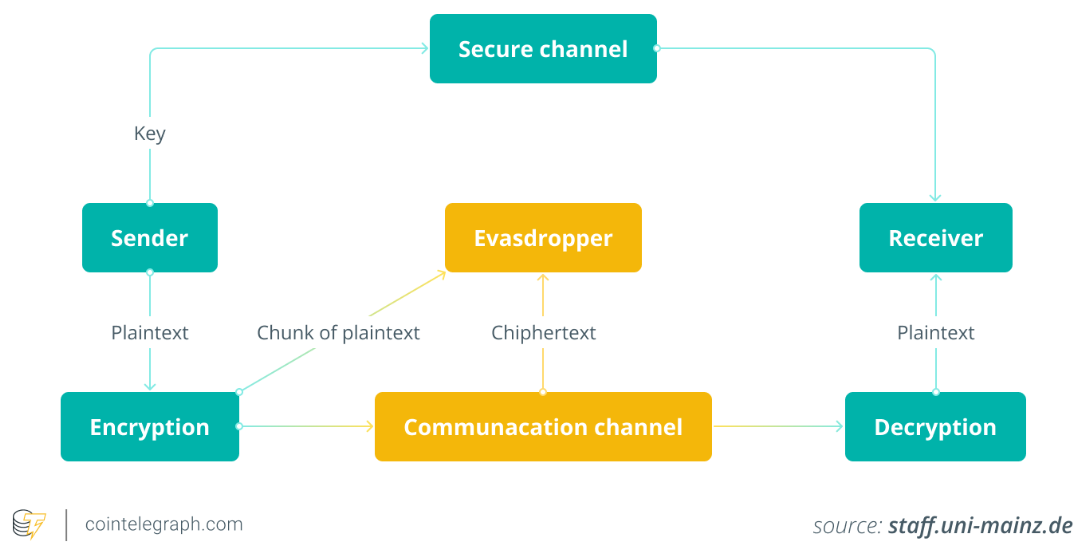
\includegraphics[width=0.8\linewidth, keepaspectratio]{Figures/KPA.png}
    \caption{A visual representation of how an attacker can acquire pairs of plaintexts and ciphertexts in a KPA \cite{cointelegraphCointelegraphBitcoin}}
    \label{fig:KPA}
\end{figure}

\subsubsection{Chosen Plaintext Attack}
Unlike with COAs and KPAs a chosen plaintext attack (CPA) doesn't rely on an attacker being able to intercept messages instead, it assumes that the attacker has access to an encryption oracle (that is viewed as a black box) and is able to obtain ciphertexts for arbitrary plaintexts \cite{Katz2007-mm}. The aim of this attack is for the attack to obtain all parts of the encryption key. 

There are two variants of a CPA; batch CPA and Adaptive CPA. Batch CPA (often just called CPA) is where an attacker chooses a number of plaintexts before seeing any corresponding ciphertexts. All of the plaintexts are then sent to the oracle and all the ciphertexts are returned (in such a way that it creates pairs of plaintexts and ciphertexts). Contrastingly in an adaptive CPA (most often referred to as CPA2) an attacker can request the ciphertexts of additional plaintexts after having seen a number of plaintext-ciphertext pairs.

CPAs are generally considered more powerful than COAs and KPAs as the attacker is able to target specific terms or phrases without having to wait for them to occur naturally and be intercepted. This means that any cipher considered secure against a CPA can also be considered secure against COAs and KPAs.

\subsubsection{Chosen Ciphertext Attack}
Building upon a CPA a chosen ciphertext attack (CCA) now grants an attacker a decryption oracle (also viewed as a black box) as well as an encryption oracle and so is able to obtain plaintexts from arbitrary ciphertexts. This now allows an attacker to defeat schemes that were considered secure under CPA, for example, the El Gamal cryptosystem is semantically secure under CPA but can be trivially defeated by CCA.

Like CPAs, there are a few variants of CCAs namely; non-adaptive, adaptive and lunchtime. The non-adaptive (or batch) and adaptive variants work the same as for a CPA only using decryption rather than encryption. Where an attacker chooses the ciphertexts to be decrypted before seeing any plaintexts is non-adaptive CPA (generally just called CPA), and where an attacker may choose additional ciphertexts to decrypt after seeing some number of plaintexts is adaptive CPA (often abbreviated to CCA2). The lunchtime variant however works a bit differently and is somewhat of a combination of the two previous methods. The lunchtime variant (shortened to CCA1) allows an attacker to make adaptive chosen-ciphertext queries (as in CCA2) but only up until a certain point. After this point the attacker can no longer make queries to the oracle and may only use the information already gathered to continue the attack. The idea behind the lunchtime variant stems from the idea that an attacker may be able to access a users computer whilst they are on lunch break but as soon as the user is back they no longer have access so as to avoid suspicion.

\subsubsection{Related Key Attacks}
First proposed by Biham in \cite{jofc-1994-14102} a related key attack (RKA) is a form of cryptanalysis where an attacker can see how a cipher works under a set of initially unknown keys but where a mathematical relationship connecting the keys is known \cite{cryptoeprint:2016/1171-2}. This mathematical relationship allows the attacker to exploit certain parts of a cipher so as to obtain results that are statistically more probable to occur than random.

All of the attacks that were performed as part of this project fall into the RK-CCA2 category as both encryption and decryption oracles were used as well as utilising the related key structure.

\subsubsection{Differential Attacks}
In its broadest sense, differential attacks (or differential cryptanalysis) are the study of how differences in an input can affect the resulting differences in the output. When talking about block ciphers specifically it refers to the techniques used to trace differences through the cipher to try and discover where the cipher exhibits non-random behaviour and then exploiting those properties to retrieve the secret key \cite{10.1007/3-540-38424-3_1}. The discovery of Differential cryptanalysis is generally attributed to Biham and Shamir where in \cite{10.1007/3-540-38424-3_1} they proposed an attack on DES in the late 1980’s. However, it was later revealed by Coppersmith that IBM had known about differential cryptanalysis since 1974 \cite{5389567}. 

Differential cryptanalysis is usually a CPA meaning that an attacker must be able to obtain some ciphertext output from a set of plaintexts they have chosen. The basic version of the attack relies on pairs of plaintexts related by a constant difference (usually XOR). The attacker then computes corresponding pairs of ciphertexts and their differences hoping to discover patterns in their distributions that lead to the cipher being distinguished from random. The resulting pair of differences is called a differential. However, in the basic version of the key recovery attack, the attacker is instead trying to ascertain the secret key used in the cipher. Since its (re)discovery differential cryptanalysis has been the building block for most modern differential techniques.

\subsubsection{Boomerang Attack}
One such attack that builds upon the differential attack is known as a boomerang attack. First proposed in \cite{10.1007/3-540-48519-8_12} by Wagner in 1999 the boomerang attack splits the cipher into two consecutive stages allowing for a differential that doesn’t have to cover the entire cipher and instead only needs to cover part of it. During the attack, a so-called ‘quartet’ structure is sort after where this quartet contains four plaintexts that adhere to certain restrictions. To obtain these quartets an attacker must first choose a plaintext, A, then XOR this with some chosen differential \(\alpha\) to get a new plaintext B. After encrypting these plaintexts with the algorithm in question to obtain ciphertexts A and B these ciphertexts are then XOR'ed with a known differential \(\delta\) to obtain two new ciphertexts C and D. Ciphertexts C and D are then decrypted through the algorithm to acquire the remaining two plaintexts. If all four plaintexts fit the quartet conditions then they are said to be a right quartet,

Since its release the boomerang attack has seen lots of use and in some cases produces very good results for attacks on block ciphers as seen in \cite{inproceedings2}, \cite{AC:BirKho09}, \cite{C:DunKelWei23}. Although most of these attacks are variants of the original boomerang such as rectangle attacks or amplified boomerang attacks, they are mostly RKA. As such there have been a number of RKA's on GOST notably \cite{inproceedings2}, \cite{fse-2004-3110}, \cite{cryptoeprint:2010/111}, \cite{articleruss}. For this project \cite{cryptoeprint:2010/111} was used as a baseline related-key boomerang attack on GOST and the results were partially replicated.

\subsubsection{Sandwich Attack}
Although initially presented in 2010 by Dunkelman et al. \cite{C:DunKelSha10} the Sandwich Attack has seen very little usage over the years with the only other paper being by Jana et al. in 2019 \cite{DBLP:journals/iacr/JanaRSP23}. As such these papers are the only source of information on how the attack works. However, the sandwich attack is a follow-on from a related-key boomerang attack so some of the workings of the attack can be ascertained from that. In \cite{C:DunKelSha10} they initially describe the sandwich attack by first explaining a related key boomerang attack and then advancing into the sandwich attack. 
As mentioned before in a related key boomerang attack the cipher is split into two consecutive sections, however, in a sandwich attack the cipher is now split into three cascading sub-ciphers. A sandwich attack still utilises the sub-ciphers E0 and E1 however one of them will be one round shorter compared to the boomerang attack. This is due to the third sub-cipher, M (sometimes referred to as the filling and hence the name sandwich attack), operating on exactly one round. The round that M operates on can be taken from either E0 or E1 and is chosen based on which provides the highest probability of a specific differential appearing. The purpose of this extra round is to increase the probability of a right quartet occurring and therefore reducing the number of plaintexts needed for the attack.

Figure \ref{fig:boomsand}, shows the basic quartet structure for both a related key boomerang and a sandwich attack. From diagram b, it is clear to see where the extra middle stage has been added to the process and subsequently how it differs from the related key boomerang attack in diagram a. 

\begin{figure}
    \centering
    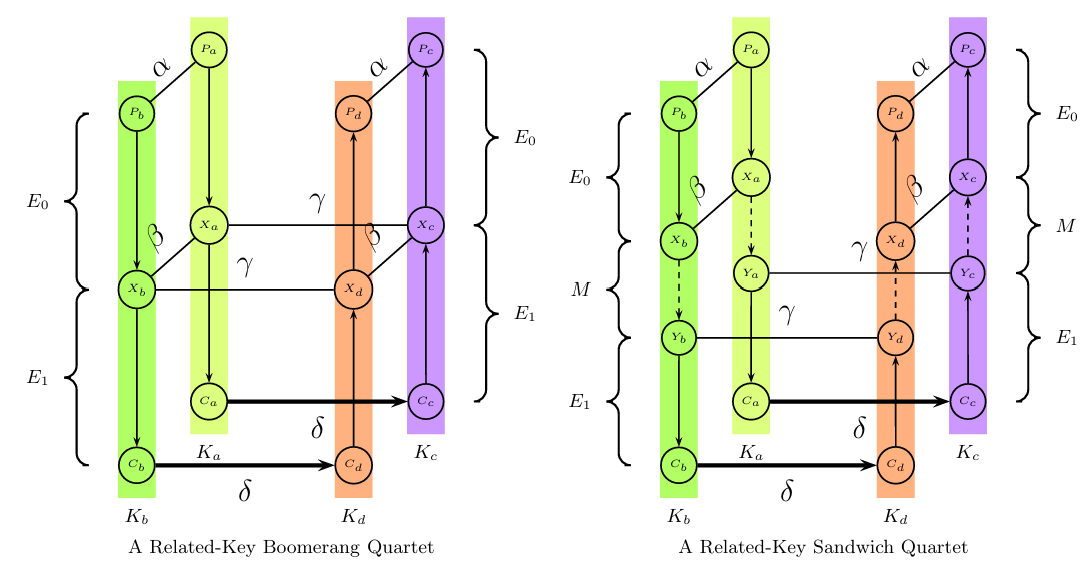
\includegraphics[width=\linewidth, keepaspectratio]{Figures/Boom_Sand_Diag.png}
    \caption{Two diagrams showing the quartet structure of a related-key boomerang attack (a - left) and a sandwich attack (b - right)\cite{C:DunKelSha10}}
    \label{fig:boomsand}
\end{figure}

\section{Methodology}
The aim of this project is to discuss the possibility of a more generalised sandwich attack specifically looking at its feasibility when used against the GOST block cipher. To aid in trying to accomplish this we have extended upon ideas discussed in the related work section by replicating the works from \cite{C:DunKelSha10} and \cite{cryptoeprint:2010/111} to provide a platform from which a sandwich attack on GOST can be built.

\subsection{A Sandwich Attack On KASUMI}
The first stage of this project was to implement the KASUMI block cipher to be able to encrypt and decrypt arbitrary data. This would be used as a black box conforming to the operations of an attack in the style of CCA2. Using this black box we would then go on to implement the sandwich attack presented in \cite{C:DunKelSha10} trying to achieve similar results and prove that the sandwich attack is a viable method of cryptanalysis.

\subsubsection{The Implementation of KASUMI}
Before implementing KASUMI it was first key to understand how it works. Utilising a 128-bit key and a 64-bit input/output, KASUMI is a relatively simple block cipher containing at its core an 8-round Feistel network. It starts by splitting the 64-bit input word into two 32-bit halves, Left and Right, with the right half containing the most significant bits and the left containing the least significant bits.

\begin{center}
    \(Input = R_0 || L_0\)
\end{center}
In each round Right is XOR'ed with the output from the round function and then the halves are swapped.
\begin{center}
    \(L_i = F_i(KL_i, KO_i, KI_i, L_{i-1}) \otimes R_{i-1}\)
    
    \(R_i = L_{i-1}\)
\end{center}
where \(KL_i, KO_i, KI_i\) are round keys for the \(i^{th}\) round.

Depending on if the round in question is even or odd, then there is a slightly different round function that is applied. In either case each round is comprised of a combination of two functions \(FL_i\) and \(FO_i\) where \(FO_i\) contains a function \(FI()\).

For an odd round:
\begin{center}
    \(F_i(K_i, L_{i-1}) = FO(KO_i, KI_i, FL(KL_I, L_{i-1}))\)
\end{center}

For an even round:
\begin{center}
    \(F_i(K_i, L_{i-1}) = FL(KL_i, FO(KO_I, KI_i, L_{i-1}))\)
\end{center}
What this essentially means is that for odd rounds the data is passed through \(FL()\) then \(FO()\) whilst for even rounds it is passed through \(FO()\) then \(FL()\).

The output of each round function is a concatenation of the outputs of the previous round.

For the FL function an input of a 32-bit data string, \(I\), and a 32-bit subkey, \(KL_i\). The subkey is split into two subkeys such that:

\begin{center}
    \(KL_i = KL_{i,1} || KL_{i,2}\)
\end{center}
and the input is split into two halves \(L, R\) where \(I = L || R\). 

The output to the FL function is the 32-bit value \((L'||R')\) where:

\begin{center}
    \(R' = R \otimes ROL(L \cap KL_{i,1})\)

    \(L' = L \otimes ROL(R \cup KL_{i,2})\)
\end{center}
and where \(ROL()\) is a 16-bit rotate left.

The \(FO()\) function takes as input a 32-bit data string, \(I\), and two 48-bit sets of subkeys \(KO_i\) and \(KI_i\). The data input is split into two halves, \(I = L_0||R_0\) and the 48-bit subkeys are subdivided into three 16-bit subkeys defines as:
\begin{center}
    \(KO_i = KO_{i,1}||KO_{i,2}||KO_{i,3}\)

    \(KI_i = KI_{i,1}||KI_{i,2}||KI_{i,3}\)
\end{center}

Then for each integer \(1 \leq j \leq 3\) it is defined as:
\begin{center}
    \(R_j = FI(L_{j-1} \otimes KO_{i,j}, KI_{i,j}) \otimes R_{j-1}\)

    \(L_j = R_{j-1} \)
\end{center}

The output of the \(FO()\) function is the 32-bit value \((L_3||R_3\).

The \(FI()\) function used within the \(FO()\) function is used to pass the 16-bit input data through two S-boxes, S7 and S9. Unlike the other functions the \(FI()\) function splits the input data and key unequally with a 9-bit and a 7-bit component. After performing some operations so as to provide non-linearity to the encryption process the \(FI()\) function then returns a 16-bit value.

These functions are then combined to create the round function which is performed eight times before returning a 64-bit output string. The diagrams showcasing how the KASUMI block cipher works can be found in Figures \ref{fig:kasumi-main}, \ref{fig:kasumi-FO}, \ref{fig:kasumi-FI} and \ref{fig:kasumi-FL} of Appendix \ref{appendix:KASUMI}.

With an understanding of how KASUMI worked we then set out to create our own implementation of it which we could manipulate for use with the sandwich attack. Although the code provided in \cite{kasumispec} is written in the C programming language it was decided during the planning phase of this project that we wanted to program using Python as this was a more familiar language. Subsequently the plan was to translate the provided C code into Python so that we could have a Python implementation of KASUMI which would hopefully be easier to use and manipulate when it came to implementing the sandwich attack. 

Despite the initial development process appearing to go well, we soon ran into issues with the KASUMI implementation. Specifically we experienced issues with it not being able to provide correct encryptions. After spending a reasonable amount of time unsuccessfully being able to debug the implementation of KASUMI it was decided that in the interest of trying to maintain on schedule a pre-existing implementation of KASUMI would be used. Although this would likely make the modifications needed to implement the sandwich attack harder to implement, we decided that a known to be working KASUMI implementation would be more beneficial and would also save a significant portion of time we would have otherwise had to send on debugging our original attempt to implement the cipher. The working implementation we chose to incorporate into our project came from \cite{asecuritysite_82320} and we experienced no issues with this when testing encryption or decryption functions.
 
\subsubsection{The Implementation of a Sandwich Attack on KASUMI}
With the implementation of KASUMI working we were then able to progress onto building the sandwich attack. The initial step was to modify the KASUMI code so that it would be able to perform as a black box and provide all the information necessary to undertake a sandwich attack. Although we speculated that this may prove difficult due to not using an implementation of KASUMI that we had written, it proved to be relatively simple to incorporate the extra functions. Mainly this section consisted of manipulating KASUMI so that it only operated on seven rounds rather than eight as the attack presented in \cite{C:DunKelSha10} proposes a distinguisher for 7-round KASUMI and then utilises brute force methods for the final round. We also needed to add in new function calls to provide us with the intermediate values from the sub-cipher M, see Figure \ref{fig:boomsand}.

Next we moved onto implementing the quartet conditions which are the bulk of the sandwich attack implementation. Utilising the pseudocode provided in \cite{C:DunKelSha10} we were quickly able to add the conditions into the project and begin testing. However, once testing began we soon realised that none of the conditions were being met despite \cite{C:DunKelSha10} suggesting that we should be seeing a right quartet, all three conditions being met, with probability \(1/4\). After spending a long time trying to debug the code, we were unable to find any notable differences between our work and the pseudocode presented in \cite{C:DunKelSha10}. This was suggesting that the work presented in \cite{C:DunKelSha10} may not have been correct and was not replicable. However, we were later able to establish that the paper provided on the official International Association for Cryptologic Research (IACR) website was an outdated file containing a preprint paper which had not been moderated and so subsequently contained a number of errors. This meant that all of the implemented code at the time was wrong and would explain why we were experiencing so many issues trying to find right quartets. Due to these errors found in the paper we had access to, we then had to search for the most up-to-date version of the paper which proved quite difficult. However, we were eventually able to find a corrected paper, \cite{jofc-2014-25962}, which contained the correct form for the quartet conditions. From this new paper we were then able to successfully implement the sandwich attack on KASUMI although due to the issues surrounding the paper this took far longer than expected and put the project quite far behind schedule.

\subsection{A Related-Key Boomerang Attack On GOST}
The next stage of this project was to go on to replicate the related-key boomerang attack presented in \cite{cryptoeprint:2010/111} in a similar way to how we implemented the sandwich attack on KASUMI. That is, creating a black box implementation of GOST to use in a related-key CCA2 style boomerang attack. The reasoning behind implementing a related-key boomerang attack on GOST is because we believe it will provide a useful mid-point between the previously implemented sandwich attack on KASUMI and the proposed sandwich attack on GOST. This mid-point can then be used as a stepping stone to help guide the project towards answering the research question.

It is important to note at this stage that the variant of boomerang attack on GOST that is implemented as part of this project originally comes from \cite{unfindable} however, we have been unsuccessful in being able to locate this paper and so we utilise \cite{cryptoeprint:2010/111} instead as this paper replicates the work from \cite{unfindable} and provides pseudocode useful for the project. As part of this project we do not go on to implement any of the advanced techniques presented in \cite{cryptoeprint:2010/111} as we felt it was only necessary to use a 'basic' boomerang attack on GOST given it is only being used as a stepping stone towards an implementation of a sandwich attack on GOST.

\subsubsection{The Implementation of GOST}
Although a more complex block cipher than KASUMI due to it being a 32-round balanced Feistel network structure, the functionality of GOST is much more simple, specifically when talking about the round function. Figure \ref{fig:GOST} shows a diagram for how the GOST round function works which is as follows: Let \(L\) and \(R\) be the 32-bit halves of the input to a round (GOST takes as input 64-bit data word and 256-bit key). A 32-bit round key modulo \(2^{32}\) is then added to \(R\), \(R = R + K_i\). This new value then has eight 4-bit S-boxes applied to it and the result after this is the left-shifted by eleven bits. Finally, this value is then XOR'ed with \(L\) to produce a new left half. As with most Feistel network structures the results from the round function (the newly calculated value for \(L\) and the unchanged \(R\)) are swapped. A diagram showing a singular round and the full operation of GOST can be found in Figures \ref{fig:gost1r} and \ref{fig:gost32r} of Appendix \ref{appendix:GOST}. Another key detail of GOST is that it operates in two components; the first 24 rounds and the last 8 rounds. The only difference between these sections is that the ordering of the subkeys is reversed for the final 8 rounds.

\begin{figure}[hbt!]
    \centering
    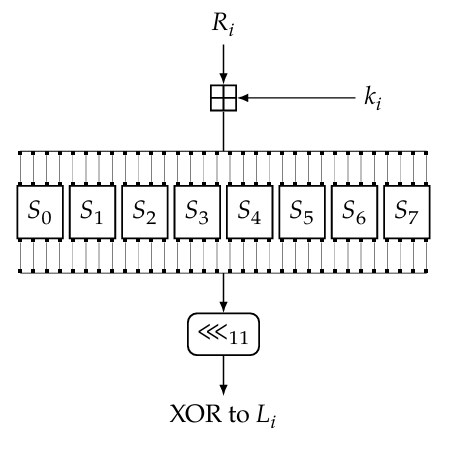
\includegraphics[width=1\linewidth]{Figures/GOST.png}
    \caption{A diagram showing how the GOST round function works \cite{cryptoeprint:2016/1171-141}}
    \label{fig:GOST}
\end{figure}

Although the original plan was to implement an original version of GOST written in Python, due to the setbacks experienced whilst developing the new Python implementation of KASUMI we decided it was best to use a pre-made solution so as to prevent any further setbacks and help to get the project back on schedule. The existing solution we used came from \cite{githubGitHubBozhuGOSTPython} and we experienced no issues surrounding the incorporation of this into the project and were able to successfully get both the encryption and decryption sides of the cipher to work without fault. 

It should be noted here that unlike KASUMI, which uses a fixed set of S-boxes, GOST is able to use a variety of S-boxes of varying strengths. It is said that this was included as a feature by the Russian Government (who have used variations of GOST as their encryption standard since the 1970's) so that they could provide 'weaker' S-boxes to Russian companies and corporations who they wished to spy on whilst giving the stronger S-boxes to those that held sensitive information that they did not want to be leaked. As such, for this project we will be utilising the S-boxes defined in \cite{doi:https://doi.org/10.1002/9781119183471.ch14} as these are generally considered the standard S-boxes. Despite the fact we have defined the specific S-boxes used in this project we later realised that the related-key boomerang attack, and subsequently the sandwich attack, on GOST are S-box agnostic meaning that the attack should work for any set of S-boxes and not just the ones we have defined.

\subsubsection{The Implementation of a Related-Key Boomerang Attack On GOST}
After successfully implementing the existing GOST code we then moved on to incorporating the related-key boomerang attack from \cite{cryptoeprint:2010/111} into the project. The first stage was to manipulate the GOST implementation into a black box suitable for the related-key boomerang attack. As with modifying KASUMI into a black box we expected this to be troublesome as the GOST implementation was not code we had written and so might not be best suited to being moulded the way we needed. Although it was more difficult to add in the extra functions that were needed compared to KASUMI, this process was still easier than we had anticipated. This section mainly focussed on creating a function to return the value after the first 24 rounds but before the last 8 rounds of the cipher as well as ensuring the cipher code worked in the same format as the attack code.

Continuing on, we then added the quartet conditions to the attack code which like the sandwich attack is a large proportion of the code needed for a boomerang attack. After including these we then set about testing the code to see if we could obtain any right quartets and establish whether \cite{cryptoeprint:2010/111} had provided a repeatable attack. However, upon starting the testing we were unable to achieve any right quartets nor were we able to successfully get plaintexts that could meet any of the quartet conditions. Thinking that this would be a similar fix to that of the sandwich attack we experimented trying to implement similar debugs but without success. After a long period of time spent trying to fix the code so that it would produce right quartets without being able to find any issue with what we had written according to \cite{cryptoeprint:2010/111} we decided to assume a 'worst-case scenario' and so then started to test the code under the assumption that the paper was wrong. We did this by performing the attack half in reverse. What this means is that we still used plaintexts \(P_a\) and \(P_b\) as before and encrypted them to obtain ciphertexts \(C_a\) and \(C_b\) respectively however, rather than then getting two new ciphertexts by differing the originals why a known value \(\delta\) we instead started with two new plaintexts \(P_c\) and \(P_d\). What this meant was that we could then encrypt all four plaintexts using their respective keys to get four ciphertexts and from this we could then see the most common differences between the pairs of ciphertexts, \((C_a, C_c)\) and \((C_b, C_d)\), and whether this lined up with the value for \(\delta\) provided by \cite{cryptoeprint:2010/111}. What we found was the the most probable differences for this stage of the attack were not the same as the provided value for \(\delta\) from \cite{cryptoeprint:2010/111}. After changing the value for \(\delta\) to the difference that occurred with the highest probability from our testing we were then able to achieve right quartets and so had managed to implement a working boomerang attack. However, we were unsure as to why the differentials provided in \cite{cryptoeprint:2010/111} did not work as it appears as though they are a somewhat common choice of differential among related-key boomerang attacks, notably \cite{fse-2004-3110} and \cite{inproceedings} both use the same differentials provided in \cite{cryptoeprint:2010/111}. Why these particular differentials did not work for the project we are unsure and could possibly be due to the implementation of GOST that we chose. Due to the issues we faced surrounding the incorrect/non-working differentials the project was put further behind schedule as it took far longer to implement the related-key boomerang attack on GOST than initially predicted.

\subsection{A Sandwich Attack On GOST}
With both of the building blocks complete we next were tasked with combining them to form a sandwich attack on GOST. However, due to the expected complexities that creating a sandwich attack on GOST would entail it was planned that we would first try to prove theoretically if it was possible and efficient before attempting an implementation. 

\subsubsection{Where to implement the filling}
The first problem we faced was where we were going to put the layer that incorporated the sandwich distinguisher. Due to the nature of GOST being split into two unequal halves (the first 24 rounds and the last 8) it seemed logical that the layer could be added in one of two places: at round 24 or at round 25 (the start of the last 8 rounds). 

\subsubsection{The Addition of Truncated Differentials}


\section{Results}
In order to establish whether the methods implemented into this project are fully functional and are able to achieve similar results to the papers they originated from, we conducted a number of tests. Specifically we show that the implementations in the project can obtain a reasonably similar number of expected quartets for a given number of trials.

\subsection{KASUMI and The Sandwich Attack}
Within \cite{jofc-2014-25962} Figure \ref{fig:ogversand} is presented showcasing the number of right quartets obtained for each of the \(100,000\) experiments that were run. These results are then compared to the expected number of right quartets which is predicted to follow a Poisson distribution with mean value eight. 

In order to obtain these results the following method is presented in \cite{jofc-2014-25962}: for each experiment generate a random quartet of keys that satisfy the relevant key differences. Then generate \(2^{16}\) plaintext quartets following the sandwich procedure. Test every plaintext quartet against the sandwich quartet conditions and note the number of quartets that meet all conditions i.e. a right quartet. This process is then to be repeated \(100,000\) times. Alongside the obtained results \cite{jofc-2014-25962} also generates the number of expected right quartets using the Poisson distribution in order to compare with their results and verify the implementations correctness. From the probability analysis undertaken in \cite{jofc-1994-14102} it was established that the probability of the related-key sandwich distinguisher (the probability of a random quartet being a right quartet) is \(2^{-14}\). So, given that each experiment contained \(2^{16}\) randomly generated quartets the expected number of right quartets (for one test), and hence the mean value used for the Poisson distribution, is calculated as \(2^{16} \cdot 2^{-14} = 4\). However, \cite{jofc-1994-14102} utilises a slight improvement to the first differential suggested in \cite{fse-2001-3046}. This improvement to the first differential fixes the value of two plaintext bits and so increase the probability of it occurring by a factor of 2 in the encryption direction. Hence the expected number of right quartets is then calculated as \(2^{16} \cdot 2^{-14} \cdot 2 = 8\) and this value is used as the mean in the Poisson distribution. As can be seen from Figure \ref{fig:ogversand} the experimental results closely follow the expected results. So, in order to verify that the implementation in this project was successful we would need to perform a similar experiment and confirm that it provided values that were close to the expected.

\begin{figure}[hbt!]
    \centering
    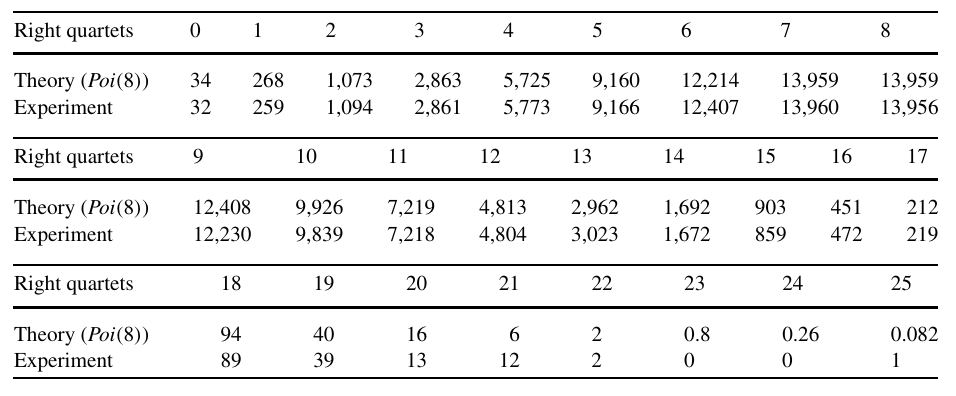
\includegraphics[width=1\linewidth]{Figures/versandogpapertable.png}
    \caption{A table showing the number of achieved right quartets against the number of expected right quartets for a sandwich attack implemented on KASUMI with \(100,000\) experiments from \cite{jofc-2014-25962}}
    \label{fig:ogversand}
\end{figure}

The implementation of this test into the project was relatively simple to do as it mostly revolved around allowing the sandwich attack to run for more than just one iteration of plaintext generation. As mentioned above, \cite{jofc-1994-14102} implemented an improvement to the differentials which resulted in the probability of a right quartet occurring increasing by a factor of two however, we elected not to incorporate this improvement as we felt that it was an unnecessary addition to the project that would add too much complexity. As such in order to calculate the expected number of right quartets we would need to use the original value for the related-key sandwich distinguisher of four as the mean for the Poisson distribution. Also, due to time restraints we have only tested the implementation in this project for \(10,000\) experiments rather than the \(100,000\) experiments as used in \cite{jofc-2014-25962}. The results for this test are summarised in Figure \ref{fig:versand} and it can be seen that the experimental results achieved for the implementation in this project closely follow the expected results to a reasonable degree of random error. Despite the significant reduction in the number of experiments performed we are still able to get results that suggest the implementation of the sandwich attack on KASUMI is correct and performs as expected. It would also be reasonable to suggest that if we were to have run our test for the full \(100,000\) experiments then the results achieved would have been similarly close or closer to the expected values. We also believe that although the differential improvement was not incorporated into the project, it would not have affected the spread of results and we still would be able to obtain results that closely follow the expected. Despite this, by not incorporating the differential improvement it does mean that we do not have a direct comparison to the results from \cite{jofc-1994-14102} potentially suggesting that there may be some slight differences that have gone unnoticed. 

\begin{figure}[hbt!]
    \centering
    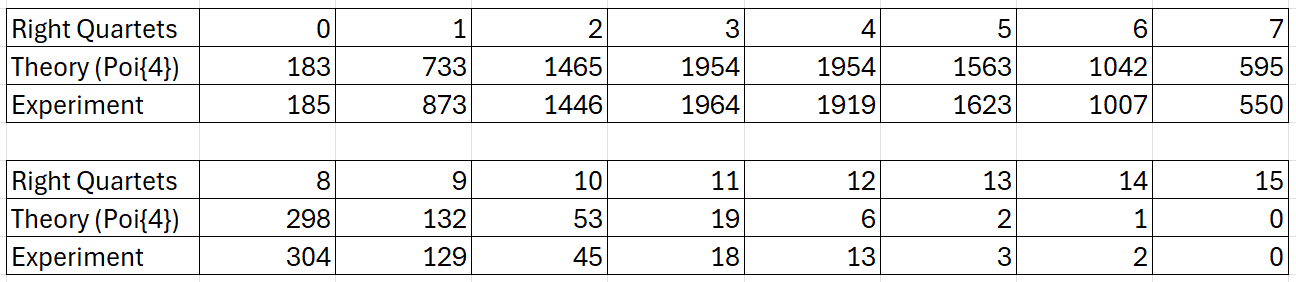
\includegraphics[width=1\linewidth]{Figures/verSandTable.png}
    \caption{The table showing the number of achieved right quartets against the number of expected right quartets for the implemented sandwich attack on KASUMI with \(10,000\) experiments}
    \label{fig:versand}
\end{figure}

\subsection{GOST and The Related-Key Boomerang Attack}
Unlike with the sandwich attack on KASUMI, \cite{cryptoeprint:2010/111} does not present any findings from a practical application of the related-key boomerang attack on GOST. What this means is that there is no evidence to compare the results from this project too and therefore have no way of validating that we have successfully implemented the related-key boomerang attack on GOST. However, as has already been established in this implementation we have had to use different differentials due to not being able to get the ones presented in \cite{cryptoeprint:2010/111} to work and so it is likely that the results we achieved would be different to those that could have been obtained from an implementation using the original differentials. Despite this we decided that we should still perform a test similar to the one used for the sandwich attack against KASUMI so as to try and see if the probability of the related-key boomerang distinguisher (the probability of a quartet being a right quartet) is correct. 

It is suggested in \cite{cryptoeprint:2010/111} that the probability of finding a related-key boomerang quartet is \(2^{-6}\). So, to try draw some similarities to the sandwich attack on KASUMI we decided to perform \(10,000\) experiments each utilising \(2^{10}\) randomly generated plaintext quartets as this meant that we could utilise a Poisson distribution with a mean value of \(4\) like the sandwich attack on KASUMI. This would at least allow for some kind of verification to take place as we would be able to compare these new results to the ones obtained previously. The rest of the testing then followed the same procedure as the one used for the sandwich attack with the only difference being that we utilised the boomerang quartet conditions instead of the sandwich ones. Part of the results table from this test is summarised in Figure \ref{fig:verboom}. The full table of results can be found in Figure \ref{fig:verboomfull} of Appendix \ref{appendix:boomerang}.

As can be seen from Figure \ref{fig:verboom} the number of right quartets achieved in the testing was significantly higher than expected. This has meant that the expected number of right quartets from the Poisson distribution with mean of \(4\) does not line up with the experimental values. Although we speculated that we may achieve slightly different values to what was expected due to using a different differential to the one used in \cite{cryptoeprint:2010/111}, we were not expecting this drastic of a difference in the values. Also included in Figure \ref{fig:verboom} is the expected number of right quartets for \(10,000\) experiments using a Poisson distribution with a mean value of \(66\). Having looked at the results we achieved, this new Poisson distribution is what we thought to be the best fit for the experimental data. Although reasonably close to the expected values, the obtained results do differ more than we would like for it to be considered a good match. However, we thought that by running more than \(10,000\) tests then the results would converge to the expected values more closely. So, we reran the experiment this time using \(100,000\) test cases. Part of the results table for this experiment is summarised in Figure \ref{fig:verboom-100k} with the full table available in Figure \ref{fig:verboomfull-100k} of Appendix \ref{appendix:boomerang}. As can be seen from the data in Figure \ref{fig:verboom-100k} the results actually appear to be more diverged from the expected values compared to the results from the experiment with \(10,000\) tests. This goes against what we were expecting and may suggest that the related-key boomerang distinguisher does not follow a Poisson distribution to predict the spread of occurring right quartets.

\begin{figure}[hbt!]
    \centering
    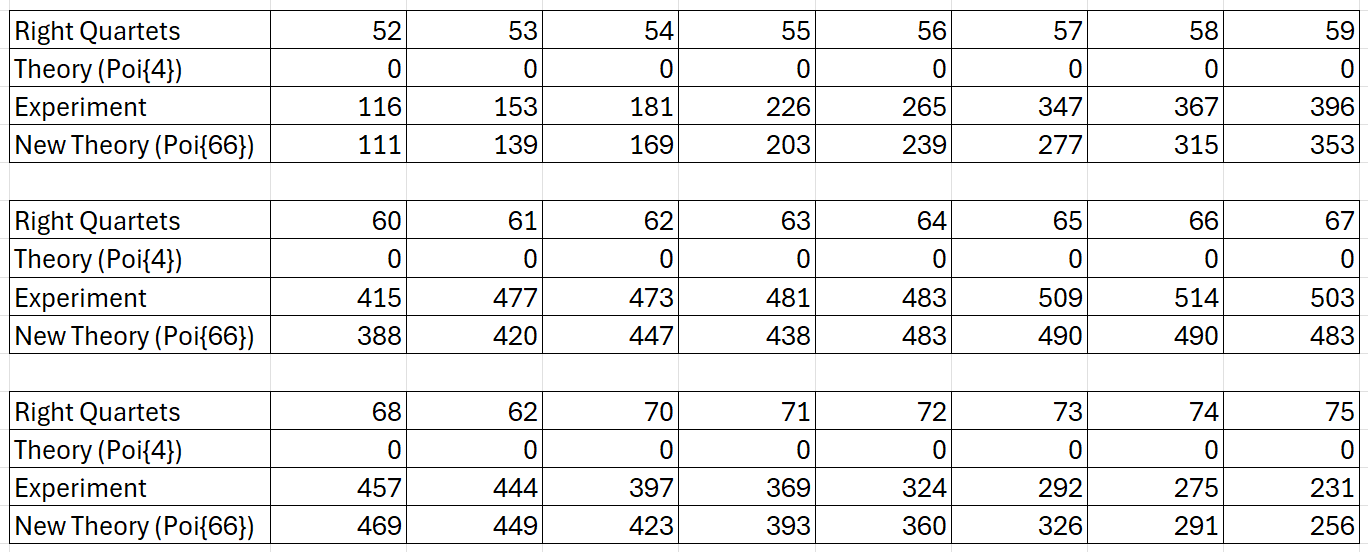
\includegraphics[width=1\linewidth]{Figures/verBoomTableMid.png}
    \caption{Part of the table showing the number of achieved right quartets, the number of expected right quartets and the true number of expected quartets for the implemented related-key boomerang attack on GOST with \(10,000\) experiments}
    \label{fig:verboom}
\end{figure}

\begin{figure}[hbt!]
    \centering
    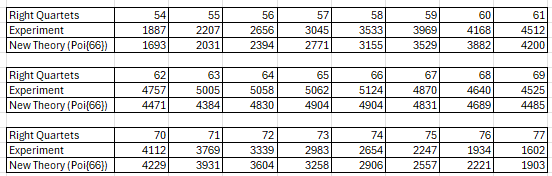
\includegraphics[width=\linewidth]{Figures/verBoomTableMid-100k.png}
    \caption{Part of the table showing the number of achieved right quartets and the number of expected right quartets for the implemented related-key boomerang attack on GOST with \(100,000\) experiments}
    \label{fig:verboom-100k}
\end{figure}

To try and establish why the results we were getting were so diverged from the expected values we generated the graphs in Figure \ref{fig:verboomg-10k} and Figure \ref{fig:verboomg-100k} showing the results from the experiment with \(10,000\) and \(100,000\) tests respectively. Comparing the two figures, we can see that the proposal we made, that running more tests should allow the experimental results to converge more to the expected results, was not strictly wrong as the spread of results in Figure \ref{fig:verboomg-100k} do more closely follow the bell curve shape of a Poisson distribution compared to Figure \ref{fig:verboomg-10k}. However, we can also now see more clearly that both sets of data appear left-skewed  in comparison to a Poisson distribution with mean of \(66\). Although in both graphs the greatest number of right quartet occurrences is for a value of \(66\) it appears as though using a Poisson distribution with a slightly lower mean value might fit the data better and present a less skewed graph. As such we have included a Poisson distribution with a mean value of \(65\) onto both graphs and this fits the data much better than the original value of \(66\).

\begin{figure}[hbt!]
    \centering
    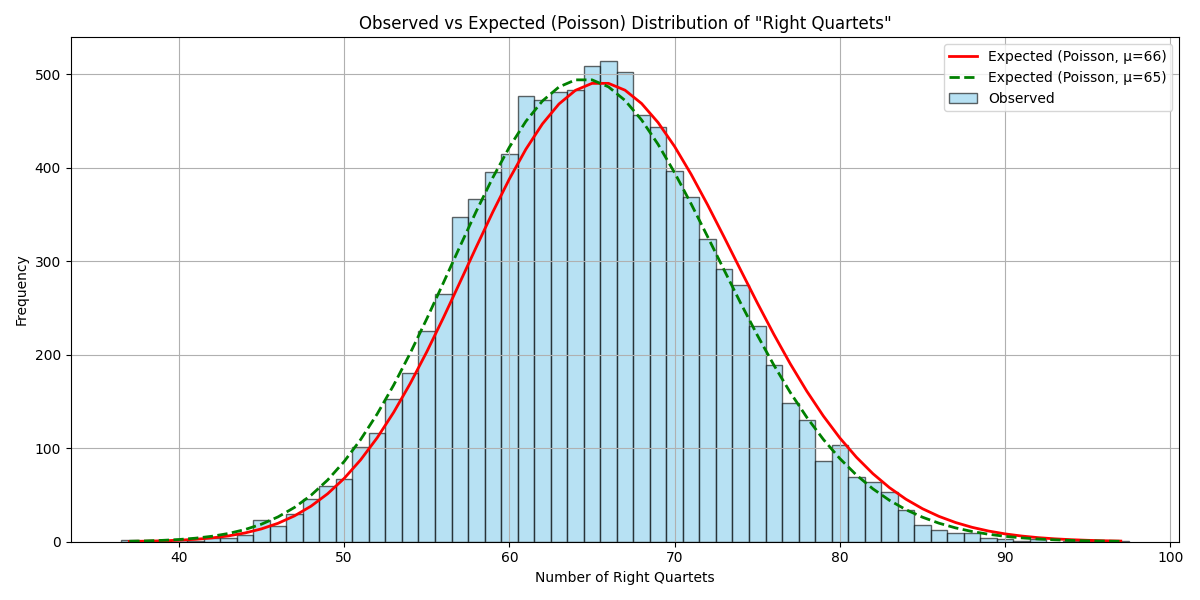
\includegraphics[width=\linewidth]{Figures/verBoomGraph.png}
    \caption{A graph showing the number of achieved right quartets against a Poisson distribution with mean 66 and mean 65 for the implemented related-key boomerang attack on GOST with \(10,000\) experiments}
    \label{fig:verboomg-10k}
\end{figure}

\begin{figure}[hbt!]
    \centering
    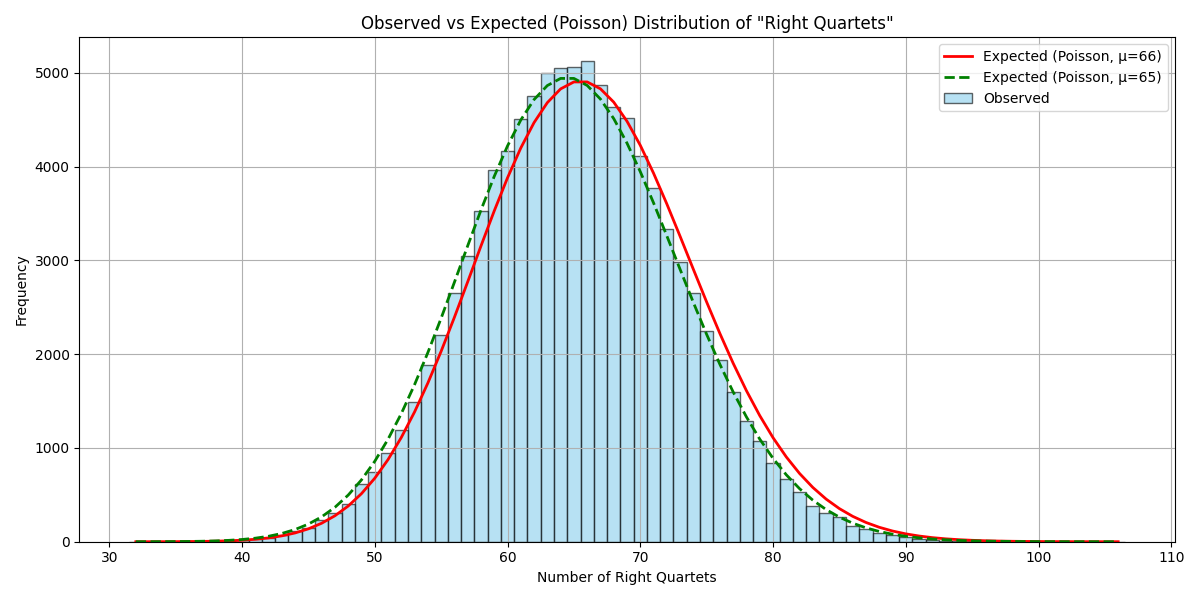
\includegraphics[width=\linewidth]{Figures/verBoomGraph-100k.png}
    \caption{A graph showing the number of achieved right quartets against a Poisson distribution with mean 66 and mean 65 for the implemented related-key boomerang attack on GOST with \(100,000\) experiments}
    \label{fig:verboomg-100k}
\end{figure}

Using this newly calculated mean value of \(65\) we next need to check the true probability of a right quartet occurring within our experiment. Taking the equation from before, rearranging it and substituting in the experimental values we get:

\begin{center}
    \(65 \div 2^{10} = P\)
\end{center}
Where \(65\) is the new mean value established for the Poisson distribution, \(2^{10}\) is the number of randomly chosen quartets per experiment and \(P\) is the probability of the related-key boomerang distinguisher. This gives a value for \(P\) of:

\begin{center}
    \(P = \frac{65}{1024} \approx 0.0635 (3.s.f) > 2^{-6}\)
\end{center}

This value of P suggests that by using the different differential in the boomerang attack compared to \cite{cryptoeprint:2010/111} we have been able to increase the probability of a right quartet occurring by more than a factor of \(4\). Although we are sceptical about this value we have been unable to find evidence to suggest that within the experiment we achieve a different probability to \(0.0635\). However, we believe that it is probably worth applying some more rigorous tests outside of this project to establish why we were unable to replicate the results from \cite{cryptoeprint:2010/111} and subsequently why the new differential we implemented appears to have increased the probability of the related-key boomerang distinguisher by a factor of \(4\).
 
\subsection{GOST and The Sandwich Attack}


\section{Evaluation}
We now look back on the research question: 'Is the sandwich attack a feasible method of breaking the GOST block cipher?' We answer this by examining the preliminary work and how its strengths and weaknesses helped to construct an idea of how to perform a sandwich attack on GOST.

\subsection{Attacking KASUMI With The Sandwich Distinguisher}
The first basic deliverable called for an implementation of a sandwich attack on the KASUMI block cipher attempting to replicate the work and results from \cite{jofc-2014-25962}. This was accomplished relatively early on on the project lifecycle although was delayed due to previously mentioned issues. We have been able to show the accomplishment of this deliverable by presenting the data in Figure \ref{fig:versand} which closely matches the expected results determined in \cite{jofc-2014-25962}. Although the algorithms used within this project have not been optimised for efficiency, we are still able to achieve right quartets for the sandwich distinguisher quickly (on average a single right quartet can be found in under thirty seconds). Despite the setbacks experienced with this section of development the implementation of the sandwich attack on KASUMI performs well and was able to achieve the predicted values when tested. However, it is worth re-mentioning that although the implementation in this project works as expected and is reasonably efficient, we did not replicate exactly the version that was implemented in \cite{jofc-2014-25962}. This was due to not implementing a change to the differentials in this project and has subsequently meant that the expected value of the sandwich distinguisher in this project is a factor of two lower than in \cite{jofc-2014-25962}. This accompanied with the fact that we did not utilise as many test cases as \cite{jofc-2014-25962} leads to some cause for doubt as to the validity of the implementation in this project as we have had no exact data to compare to and to verify what we have done. Nevertheless we believe that the data that has been produced from the implementation in this project is sufficient to say that we have successfully created a simplified version of the algorithm produced in \cite{jofc-2014-25962}. Also, we can then say that, based on the statistical analysis presented in \cite{jofc-2014-25962} from which we have generated a set of expected values, the implementation in this project is valid as it is produces results sufficiently close to these expected values.

\subsection{Attacking GOST With The Related-Key Boomerang Distinguisher}
The second basic deliverable called for an implementation of a related-key boomerang attack on the GOST block cipher attempting to implement the algorithm presented in \cite{cryptoeprint:2010/111}. This was accomplished later on into the project lifecycle than was planned due to a number of issues occurring which stalled progress. One such issue, resulted in the differentials needing to be changed from those proposed in \cite{cryptoeprint:2010/111} because we were unable to get those specific differentials to work within our project. Although \cite{cryptoeprint:2010/111} did not implement the algorithm presented and as such had no experimental data which we could use to verify the implementation from this project, we were able to generate a similar test to the one performed for the sandwich attack on GOST. The results from this data however did not line up with the values we were expecting based on the theory presented in \cite{cryptoeprint:2010/111}. In fact the solution presented in this project appeared to show an increase by a factor of four for the probability of the related-key boomerang distinguisher. This increase in the probability is potentially due to the use of different differentials within this project however, we were unable to establish an exact cause. Despite this the methods implemented in this project for the related-key boomerang distinguisher on GOST are reasonably efficient with a single right quartet being found consistently in under a second. Given that we were unable to replicate the expected values from \cite{cryptoeprint:2010/111} within this part of the project it is reasonable to assume that there exists some inconsistency. Whether that be within the implementation itself or with the original design of the algorithm, we are unsure. However, it is worth noting that despite not being able to replicate \cite{cryptoeprint:2010/111} we were still able to develop a working implementation albeit if we are unable to prove its validity.

\subsection{Attacking GOST With The Sandwich Distinguisher}
With both of the basic deliverables complete we could then utilise the information we had gained from them to begin the intermediate deliverable which asked for some form of proof that the sandwich attack would be a feasible method for breaking the GOST block cipher. This section was key to answering the research question. The analysis of how the sandwich distinguisher could be applied to GOST was accomplished very late into the project due to the issues with the basic deliverables. However, we were able to establish that through the use of truncated differentials, the sandwich distinguisher could be applied to GOST. As such we were also able to work out that by using truncated differentials and applying the 'filling' layer to the 25th round of GOST, the probability of the sandwich distinguisher on GOST would be at least as good as the related-key boomerang distinguisher. What this means is that the probability of a sandwich quartet occurring is the same as that of a related-key boomerang distinguisher. So, this allowed us to answer the research question as if the sandwich distinguisher on GOST had the same expected value for a given number of randomly generated plaintexts as the related-key boomerang distinguisher then no extra time or memory requirements would be necessary. This suggests that in theory the sandwich attack is a feasible method of breaking the GOST block cipher as it requires no more time, memory or plaintext quartets compared to a related-key boomerang attack on GOST and so answers the research question. 

\subsection{The Approach}
The approach we took towards the project centred heavily around developing existing techniques to use as stepping stones towards the larger goal of trying to answer the research question: 'Is the sandwich attack a feasible method of breaking the GOST block cipher?' For the most part this worked quite well, developing the sandwich attack on KASUMI from \cite{jofc-2014-25962} and the related-key boomerang attack on GOST from \cite{cryptoeprint:2010/111} allowed for us to gain a deeper understanding of the attacks. This understanding then helped when deciphering whether the sandwich attack would be applicable to GOST because we were able to utilise techniques and knowledge that had been gained from implementing the attacks prior. However, we did experience a number of setbacks throughout the course of this project which hindered the structured development of the solution. Notably we encountered the majority of the projects issues when developing the related-key boomerang attack on GOST. These hindrances have meant that some of the more advanced deliverables that we had initially planned to undertake have not been completed. As such, if we were given the opportunity to repeat this work then we would not change the structure of the approach in terms of replicating attacks to use as a baseline but, would change the focus of it to be more centred around developing new techniques rather than replicating old ones. We would also perform a more in-depth analysis of the papers we wished to replicate to ensure that the number of issues encountered could try to be lessened. Following on from this it may also be a good idea to allow more time to complete sections of the project as this project has run quite a bit over schedule due to unforeseen issues and subsequently has meant that we have been unable to complete everything we set out to do at the start.

\section{Conclusion}
As the final section of this project we: summarise the methods of the solution that have been presented, discuss the importance of the work undertaken and we also go on to make some suggestions towards future work that could be presented as a follow on from this project.

\subsection{Project Conclusions}
To summarise what we have presented in this paper, we first started by replicating one of the few instances of a sandwich attack, onto the KASUMI block cipher as presented in \cite{jofc-2014-25962}. Despite some setbacks we were able to achieve results that were sufficiently similar to those presented in \cite{jofc-2014-25962} to be able to say that: the sandwich distinguisher is a viable method for providing right quartets for use in an attack and that the results presented in \cite{jofc-2014-25962} were repeatable.

We then went on to create an implementation of the related-key boomerang attack presented in \cite{cryptoeprint:2010/111}. However, we soon came to realise that at least one of the implementation for this project or \cite{cryptoeprint:2010/111} contained some issues as we were unable to obtain results that fit the expected theory. Although, after we implemented a change to the differentials used in the related-key boomerang distinguisher we were able to obtain results that suggest we had improved the probability of this distinguisher by a factor of four but we were unable to verify these claims as we had no reference data to compare to. What this meant was that we were able to create a related-key boomerang distinguisher that could efficiently identify right quartets but we were unable to verify this implementations validity nor were we able to show that the theory presented in \cite{jofc-2014-25962} was correct in practice.

Finally, we analysed the possibility of applying the sandwich distinguisher to the GOST block cipher. During this we were able to notice that, through the use of truncated differentials and the specific placement of the 'filling' layer within GOST, we could apply the sandwich distinguisher to GOST with no extra cost when compared to the related-key boomerang distinguisher. Subsequently this allowed us to answer the proposed research question, 'Is the sandwich attack a feasible method for breaking the GOST block cipher?', by saying that, yes the sandwich attack is a feasible method for breaking the GOST block cipher as it should in theory have no extra requirements compared to a related-key boomerang attack which is an already known and well studied attack. Although we were unable to progress onto creating an implementation of the sandwich attack on GOST, due to the many issues experienced throughout the project, We were still able to successfully answer the research question despite not being able to experimentally verify the proposal.

\subsection{Further Work}
Based on the findings presented in this project there are a number of ways in which you could extend the work we have produced which are summarised below. 

The first point that we suggest for further work is to undertake the deliverables for this project that were not completed, namely the implementation of the sandwich distinguisher on GOST. With this implementation the theory presented in this project could be verified and thus cementing the sandwich distinguisher as a viable method for use against GOST. Also it would help to validate the claim that the sandwich attack is a feasible method for breaking the GOST block cipher and further answering the research question presented in this project.

As mentioned in the Results section, when implementing the related-key boomerang attack presented in \cite{cryptoeprint:2010/111} we were unable to replicate the theoretical findings and instead produced an implementation that appears to work with increased probability. As such we think that it would be worth double checking the findings we presented to see if they are valid and on top of this verifying whether the theory in \cite{cryptoeprint:2010/111} is incorrect as we suspect or if it is the case that the implementation in this project contains some errors.

Another way in which you could build directly on this project would be to implement the full key recovery attacks for both the sandwich and related-key boomerang distinguishers presented in this project. As has already been mentioned, within this project we have only implemented the distinguishers for each of the proposed attacks rather than the full key recovery variants as it was thought that the key recovery variants would be too complex and add too much time onto the already busy project schedule. As such, an extension of the work in this project would be to implement the key recovery attacks showing that the distinguishers would work in practice as part of a proper attack on the respective block ciphers. Although the full key recovery attack for the sandwich attack on KASUMI was implemented in \cite{jofc-2014-25962}, we believe it would still be worth while creating a new implementation of that attack to verify the claims made in \cite{jofc-2014-25962}.

The final way in which we think this work could be extended relates to the process of generalising the sandwich attack. When the sandwich attack was first presented in \cite{jofc-2014-25962} it was suggested in the 'Future Work' section that finding generic structures in which the sandwich attack is applicable was a key point of interest. In this project we have taken a step towards this generalisation by showing that the sandwich attack can be applied to GOST in theory but did not go on to provide any further generalisation. As such, if the sandwich attack could be fully generalised, and then subsequently applied to ciphers such as AES, we could see an improvement in the best known attacks for some of the strongest ciphers that currently exist.

We conclude this paper with a formal statement of the directions for further research raised above.

\begin{itemize}
    \item Problem 1: Develop an implementation for the sandwich distinguisher on GOST.
    \item Problem 2: Verify the results of the related-key boomerang distinguisher from this paper and attempt to validate the claims made in \cite{cryptoeprint:2010/111}.
    \item Problem 3: Develop implementations of the distinguishers presented in this project.
    \item Problem 4: Attempt to generalise the sandwich attack for use on generic block ciphers.
\end{itemize}


% The page lengths given for each section are indicative and will vary from project to project but should not exceed the upper limit. A summary is shown in Table \ref{table_2}.

% \begin{table}[!t]
% \renewcommand{\arraystretch}{1.3}
% \caption{Summary of Page Lengths for Sections}
% \label{table_2}
% \centering
% \begin{tabular}{cc}
% \hline\hline
% Section & Number of Pages\\
% \hline
% I. Introduction & 2\\
% II. Related Work & 2-3\\
% III. Methodology & 4-6\\
% IV. Results & 2\\
% V. Evaluation & 1-2\\
% VI. Conclusion & 1\\
% \hline\hline
% \end{tabular}
% \end{table}


% trigger a \newpage just before the given reference
% number - used to balance the columns on the last page
% adjust value as needed - may need to be readjusted if
% the document is modified later
%\IEEEtriggeratref{8}
% The "triggered" command can be changed if desired:
%\IEEEtriggercmd{\enlargethispage{-5in}}

% references section

% can use a bibliography generated by BibTeX as a .bbl file
% BibTeX documentation can be easily obtained at:
% http://mirror.ctan.org/biblio/bibtex/contrib/doc/
% The IEEEtran BibTeX style support page is at:
% http://www.michaelshell.org/tex/ieeetran/bibtex/
%\bibliographystyle{IEEEtran}
% argument is your BibTeX string definitions and bibliography database(s)
%\bibliography{IEEEabrv,../bib/paper}
%
% <OR> manually copy in the resultant .bbl file
% set second argument of \begin to the number of references
% (used to reserve space for the reference number labels box)

\newpage
\bibliographystyle{plain}
\bibliography{abbrev1,crypto,refs}



\newpage
\begin{appendices}
\section{KASUMI}\label{appendix:KASUMI}
Four figures showing diagrams of how the functions that make up the KASUMI block cipher work.

\begin{figure}[H]
    \centering
    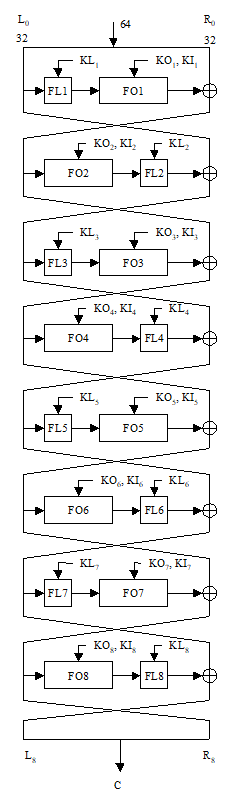
\includegraphics[width=\linewidth, height=0.85\textheight, keepaspectratio]{Figures/kasumi_diag.png}
    \caption{A figure showing the workings of the main KASUMI function}
    \label{fig:kasumi-main}
\end{figure}

\begin{figure}[H]
    \centering
    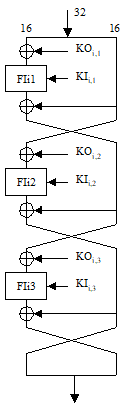
\includegraphics[width=\linewidth, height=\textheight, keepaspectratio]{Figures/FO_diag.png}
    \caption{A figure showing the workings of the FO function from KASUMI}
    \label{fig:kasumi-FO}
\end{figure}

\begin{figure}[H]
    \centering
    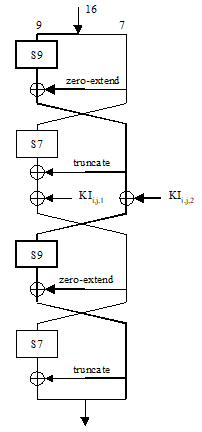
\includegraphics[width=\linewidth, height=\textheight, keepaspectratio]{Figures/FI_diag.png}
    \caption{A figure showing the workings of the FI function from KASUMI}
    \label{fig:kasumi-FI}
\end{figure}

\begin{figure}[H]
    \centering
    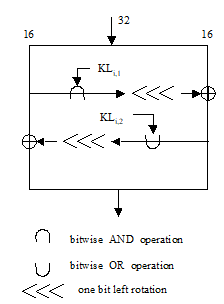
\includegraphics[width=\linewidth, height=\textheight, keepaspectratio]{Figures/FL_diag.png}
    \caption{A figure showing the workings of the FL function from KASUMI}
    \label{fig:kasumi-FL}
\end{figure}

\newpage
\section{GOST}\label{appendix:GOST}
Figures showing a diagram of one round and 32 rounds of the GOST block cipher.

\begin{figure}[H]
    \centering
    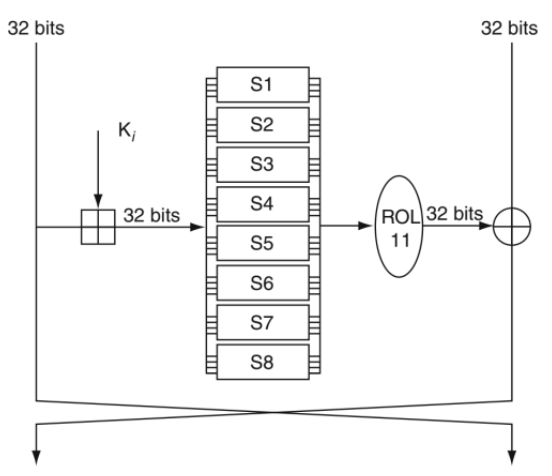
\includegraphics[width=\linewidth, height=\textheight, keepaspectratio]{Figures/gost_1r.png}
    \caption{A figure showing the workings of one round of GOST from \cite{van2011encyclopedia}}
    \label{fig:gost1r}
\end{figure}

\begin{figure}[H]
    \centering
    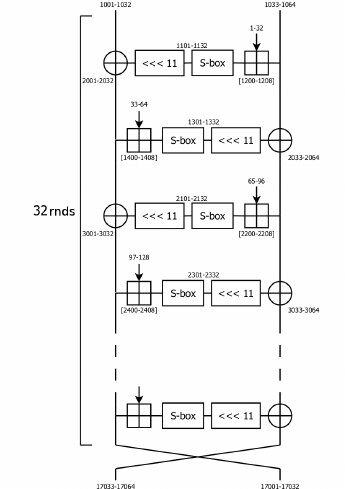
\includegraphics[width=\linewidth, height=\textheight, keepaspectratio]{Figures/gost_32r.png}
    \caption{A figure showing the workings of 32 rounds of GOST from \cite{article-g32}}
    \label{fig:gost32r}
\end{figure}

\newpage
\section{Boomerang Attack}\label{Figures/appendix:boomerang}

Figures showing the full table of results from the testing of the boomerang attack on GOST using \(10,000\) and \(100,000\) tests.

\begin{figure}[H]
    \centering
    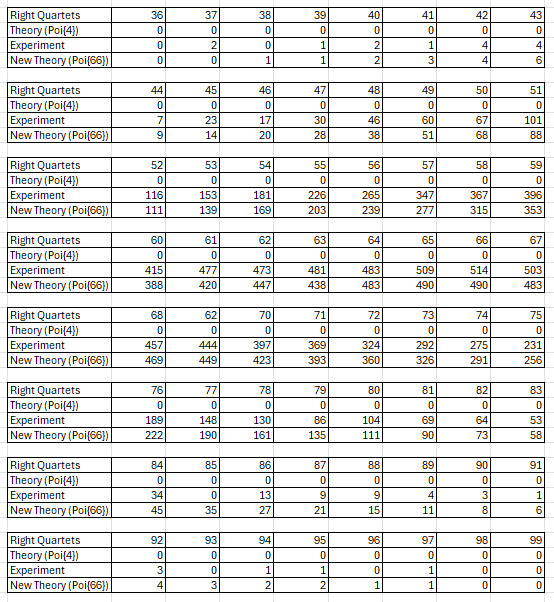
\includegraphics[width=0.9\linewidth, keepaspectratio]{Figures/verBoomTableFull.png}
    \caption{The table showing the number of achieved right quartets, the number of expected right quartets and the true number of expected quartets for the implemented related-key boomerang attack on GOST with \(10,000\) experiments}
    \label{fig:verboomfull}
\end{figure}

\begin{figure}[H]
    \centering
    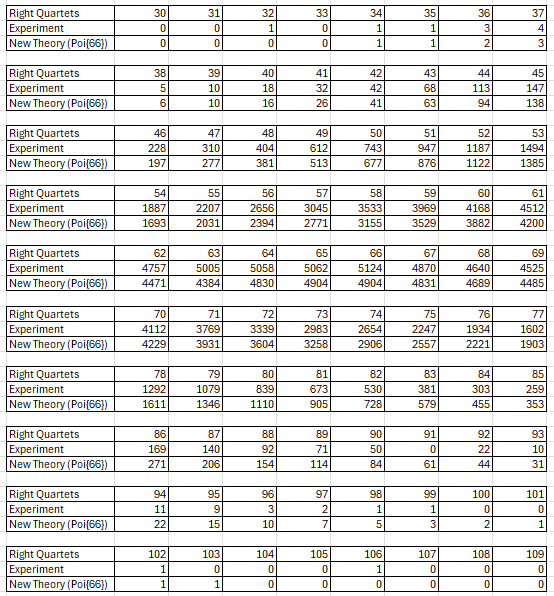
\includegraphics[width=0.9\linewidth, keepaspectratio]{Figures/verBoomTableFull-100k.png}
    \caption{The table showing the number of achieved right quartets and the number of expected right quartets for the implemented related-key boomerang attack on GOST with \(100,000\) experiments}
    \label{fig:verboomfull-100k}
\end{figure}

\end{appendices}
% that's all folks
\end{document}


